\section{Results}
\subsection{Comparison of Compute Resource Utilization}
While the performance testing is focused on comparing the overall Istio system resource utilization of sidecar and ambient modes, a quick look at one of the microservice pod resource consumptions in both modes is a good starting point.

\begin{figure}[ht!]
    \centering
    \caption{Pod memory use in Istio sidecar mode}
    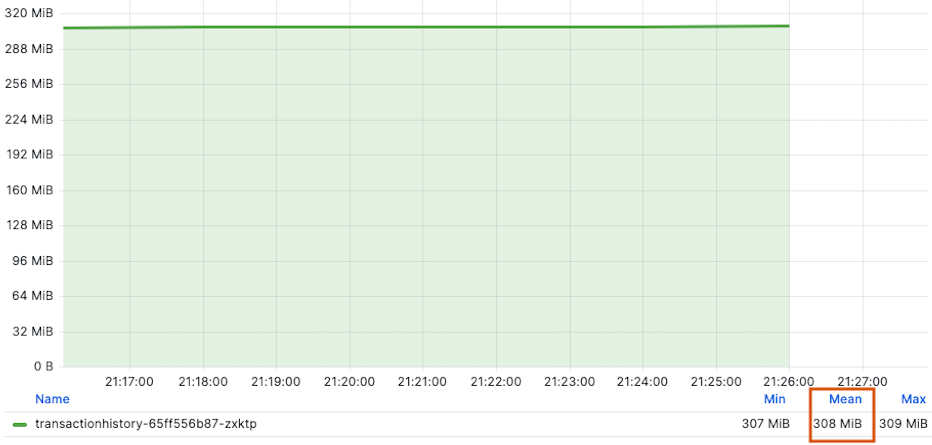
\includegraphics[width=0.95\linewidth]{resources/sidecar-pod-mem.png}
    \label{result:podMemUseSidecar}
\end{figure}

\begin{figure}[ht!]
    \centering
    \caption{Pod memory use in Istio ambient mode}
    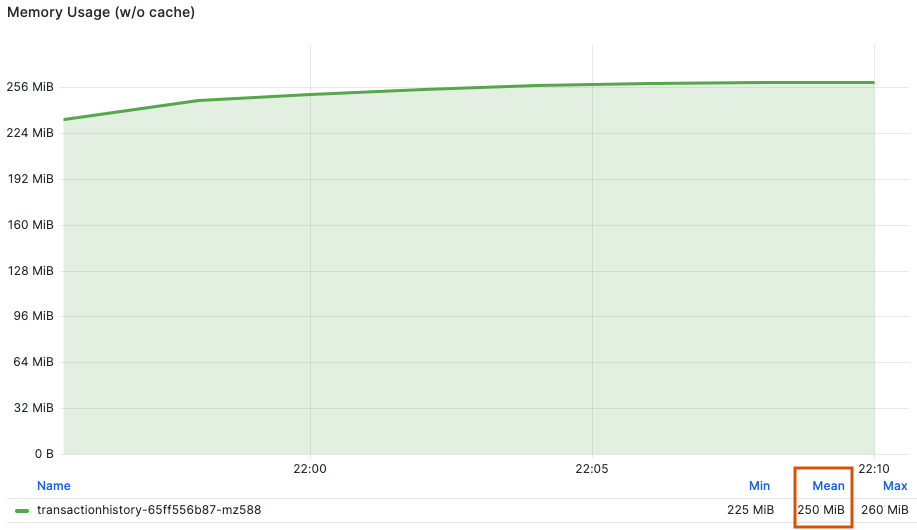
\includegraphics[width=0.95\linewidth]{resources/ambient-pod-mem.png}
    \label{result:podMemUseAmbient}
\end{figure}

Figure \ref{result:podMemUseSidecar} and \ref{result:podMemUseAmbient} shows a 10 minutes memory usage monitoring graph from Grafana for transaction history microservice pod. The result shows an improvement of 23.2\% in memory usage in Istio ambient mode with no difference in CPU usage.

\subsubsection{Istio System Resource Utilization with Single Namespace}
Istio system performance is first tested with a typical small organization deployment model by deploying all microservices in a single Kubernetes namespace 'boa'. Lets look at some configurations before jumping into the results.

In Istio standard mode, 14 pods were deployed  with:
\begin{itemize}
    \item 2 sidecars for two 2 microservices (accounts-db, ledger-db) deployed as StatefulSet x 1 replica
    \item 12 sidecars for 6 other microservices deployed as Deployment x 2 replicas
    \item Pods were distributed among 3 nodes with e2-standard-2 machine type including 2 vCPUs and 8 GiB RAM each.
\end{itemize}


\begin{figure}[ht!]
    \centering
    \caption{Istio system CPU consumption in sidecar mode}
    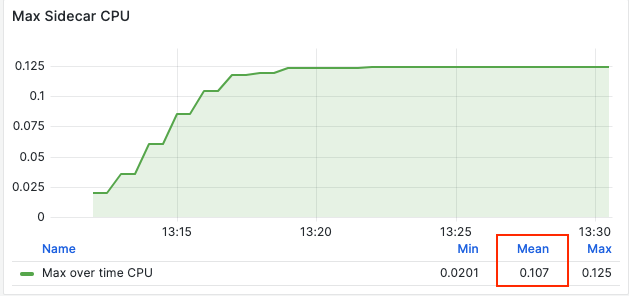
\includegraphics[width=0.9\linewidth]{resources/max-sidecar-cpu.png}
    \label{result:maxSidecarCpu}
\end{figure}

\begin{figure}[ht!]
    \centering
    \caption{Istio system Memory consumption in sidecar mode}
    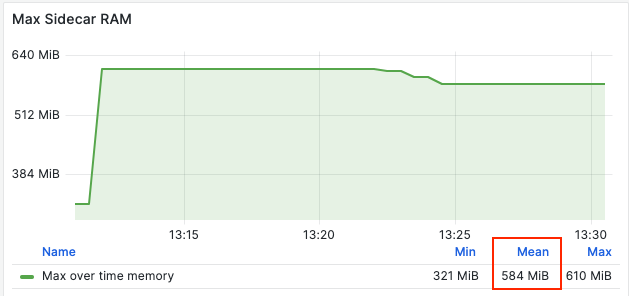
\includegraphics[width=0.9\linewidth]{resources/max-sidecar-ram.png}
    \label{result:maxSidecarRam}
\end{figure}



\begin{itemize}
    \item Pods distributed among 4 nodes with e2-standard-2 machine type including 2 vCPUs and 8 GiB RAM each.
    \item 4 instance of Ztunnel on each nodes
    \item 3 instance of Waypoint proxy when L7 proxy is engaged
\end{itemize}

As part of this test, observability stack is used to capture any microservice service downtime by tracking HTTP response code 200. 

\subsubsection{Sample Table}
\begin{table}[ht!]
\centering
    
	\caption{Comparison \textit{p} values}
	\begin{tabular}{ |l|c|c|}	
		\hline		
		\textbf{Attribute} & \textbf{\textit{p-value}} & \textbf{Significant} \\ \hline
		Model A	 & 0.0521 & N \\ \hline
		Model B  & 0.6171 & N \\ \hline 
		Model C  & <0.00001 & Y \\ \hline 
	\end{tabular}
	\label{tab:pvalues}
\end{table} 

